\section{Introduction}

Let $q \in \C^\times$ and let $\Sigma$ be an oriented surface.
We define the Kauffman bracket skein algebra (KBSA) of $\Sigma$, denoted $S_q(\Sigma)$,
as the free $\C(q)$-module spanned by diagrams of unoriented framed links
in $\Sigma$, up to planar isotopy, modulo the local relations
\begin{align}
    \scalebox{0.75}{\trivialcomponent} & = -[2]\varnothing \label{trivial} \\
    \scalebox{0.75}{\positivecrossing} & = q^{\frac12} \ \scalebox{0.75}{\verticalresolution} + q^{-\frac12} \ \scalebox{0.75}{\horizontalresolution} \label{crossing}
\end{align}
where we define $$[n] = \frac{q^n - q^{-n}}{q - q^{-1}}$$
for all positive integers $n$, and $\varnothing$ is the empty
diagram. We call the relations (\ref{trivial}) and (\ref{crossing})
the Kauffman bracket skein relations. Multiplication in $S_q(\Sigma)$
is defined on link diagrams $D_1$ and $D_2$ by stacking $D_1$
on top of $D_2$ using over crossings and extended linearly for all
elements of $S_q(\Sigma)$. For example, in $S_q(T^2)$,
the product of a meridian and a longitude is computed as
\begin{align*}
    \scalebox{0.75}{
        \begin{tikzpicture}[baseline=0]
            \draw[thick, ->>- = 0.57] (-1,-1) -> (-1,1);
            \draw[thick, ->- = 0.55] (-1,1) -> (1,1);
            \draw[thick, ->>- = 0.57] (1,-1) -> (1,1);
            \draw[thick, ->- = 0.55] (-1,-1) -> (1,-1);
            \draw[thick] (0,1) -- (0, -1);
    \end{tikzpicture}}
    *
    \scalebox{0.75}{
        \begin{tikzpicture}[baseline=0]
            \draw[thick, ->>- = 0.57] (-1,-1) -> (-1,1);
            \draw[thick, ->- = 0.55] (-1,1) -> (1,1);
            \draw[thick, ->>- = 0.57] (1,-1) -> (1,1);
            \draw[thick, ->- = 0.55] (-1,-1) -> (1,-1);
            \draw[thick] (-1, 0) -- (1,0);
        \end{tikzpicture}}
    & = 
    \scalebox{0.75}{
        \begin{tikzpicture}[baseline = 0]
            \draw[thick, ->>- = 0.57] (-1,-1) -> (-1,1);
            \draw[thick, ->- = 0.55] (-1,1) -> (1,1);
            \draw[thick, ->>- = 0.57] (1,-1) -> (1,1);
            \draw[thick, ->- = 0.55] (-1,-1) -> (1,-1);
            \draw[thick] (0,1) -- (0, -1);
            \draw[thick] (-1, 0) -- (-0.1, 0);
            \draw[thick] (0.1, 0) -- (1,0);
        \end{tikzpicture}} \\
    & = q^{\frac12} \, 
    \scalebox{0.75}{
        \begin{tikzpicture}[baseline=0]
            \draw[thick, ->>- = 0.57] (-1,-1) -> (-1,1);
            \draw[thick, ->- = 0.55] (-1,1) -> (1,1);
            \draw[thick, ->>- = 0.57] (1,-1) -> (1,1);
            \draw[thick, ->- = 0.55] (-1,-1) -> (1,-1);
            \draw[thick] plot [smooth, tension=1] coordinates {(0,1) (0.25,0.25) (1,0)};
            \draw[thick] plot [smooth, tension=1] coordinates {(-1,0) (-0.25,-0.25) (0,-1)};
        \end{tikzpicture}}
    + q^{-\frac12}
    \scalebox{0.75}{
        \begin{tikzpicture}[baseline=0]
            \draw[thick, ->>- = 0.57] (-1,-1) -> (-1,1);
            \draw[thick, ->- = 0.55] (-1,1) -> (1,1);
            \draw[thick, ->>- = 0.57] (1,-1) -> (1,1);
            \draw[thick, ->- = 0.55] (-1,-1) -> (1,-1);
            \draw[thick] plot [smooth, tension=1] coordinates {(-1,0) (-0.25,0.25) (0,1)};
            \draw[thick] plot [smooth, tension=1] coordinates {(0,-1) (0.25,-0.25) (1,0)};   
        \end{tikzpicture}}
    \end{align*}
where we represent the torus $T^2$ as a square with opposite
edges identified.

One particularly notable property of $S_q(\R^2)$ is that
it is related to the representation theory of the quantum group
$U_q(\slin_2)$. More specifically, with some modifications,
$S_q(\R^2)$ coincides with the graphical calculus of
$U_q(\slin_2)$-equivariant maps $\varphi: V_1^{\otimes n} \to V_1^{\otimes m}$
where $V_1$ and $V_0 = V^{\otimes 0} = \C$
are the fundamental and trivial representations of $U_q(\slin_2)$.
In a more down-to-earth fashion, this means that the relations
(\ref{trivial}) and (\ref{crossing}) are short hand for equations
related to evaluation map $V_1 \otimes V_1 \to V_0$, the coevaluation map $V_0 \to V_1 \otimes V_1$,
and the braiding map $V_1 \otimes V_1 \to V_1 \otimes V_1$ defined by
$x \otimes y \mapsto y \otimes x$.

The construction of $S_q(\Sigma)$ for other surfaces $\Sigma$,
then can be seen as being the answer to the question
``What happens if we draw the same kinds of pictures but on
other surfaces?'' Of course, nothing here is special to the Lie 
group $\mathrm{SL}_2$ and its Lie algebra $\slin_2$ --- we can
play this game with other Lie groups, such as $\mathrm{PGL}_2 = \mathrm{GL}_2/\sim$
where $S \sim T$ if and only if they differ up to scaling.

Now, with the representation theory of $U_q(\pgl_2)$ in mind,
one defines the $\PGL_2$ skein algebra (otherwise known as the chromatic skein algebra,
or graph skein algebra) of an oriented surface $\Sigma$, denoted $S_q^Y(\Sigma)$, 
as the free $\C(q)$-module spanned by diagrams of trivalent spatial ribbon
graphs embedded in $\Sigma$, up to planar isotopy, modulo
the following modified Yamada relations:
\begin{align}
    \scalebox{0.75}{\trivialcomponent} & = [3]\varnothing \\
    \scalebox{0.75}{\itangle} - \frac{1}{[2]} \ \scalebox{0.75}{\horizontalresolution} & = \scalebox{0.75}{\htangle} - \frac{1}{[2]} \ \scalebox{0.75}{\verticalresolution} \\
    \scalebox{0.75}{\positivecrossing} & = q^2 \ \scalebox{0.75}{\verticalresolution} + (q^{-2} - 1)\ \scalebox{0.75}{\horizontalresolution} + [2] \, \scalebox{0.75}{\itangle}\\
    \scalebox{0.75}{\monogon} &= 0.
\end{align}
Multiplication in $S_q^Y(\Sigma)$ is defined in the same way as
in $S_q(\Sigma)$.

Since the representation category of $U_q(\pgl_2)$ is a
subcategory of the representation category of $U_q(\slin_2)$,
we ought to be able to include $S_q^Y(\R^2)$ into $S_q(\R^2)$. Indeed, this
this inclusion is given by the map $JW: S_q^Y(\R^2) \to S_q(\R^2)$
defined by
 \begin{align*}
    \scalebox{0.75}{
    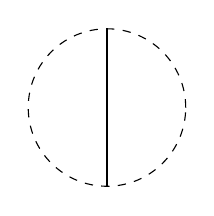
\begin{tikzpicture}[baseline=0]
        \draw[dashed] (0,0) circle (1);
        \draw[thick] (0,-1) -- (0,1);
    \end{tikzpicture}
    } & \mapsto 
    \scalebox{0.75}{
    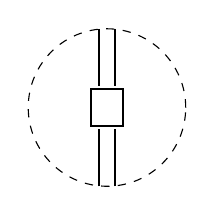
\begin{tikzpicture}[baseline=0]
        \draw[dashed] (0,0) circle (1);
        \node at (0,0) [thick,rectangle,draw] {$\phantom{2}$};
        \draw[thick] (-0.1, 1) -- (-0.1,0.27);
        \draw[thick] (0.1, 1) -- (0.1,0.27);
        \draw[thick] (-0.1, -1) -- (-0.1,-0.27);
        \draw[thick] (0.1, -1) -- (0.1,-0.27);
    \end{tikzpicture}
    } \\
    \scalebox{0.75}{
    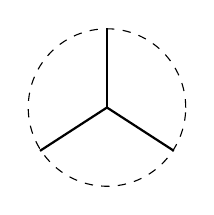
\begin{tikzpicture}[baseline=0]
        \draw[dashed] (0,0) circle (1);
        \draw[thick] (0,0) -- (0,1);
        \draw[thick] (0,0) -- (0.85,-0.55);
        \draw[thick] (0,0) -- (-0.85,-0.55);
    \end{tikzpicture}
    } & \mapsto
    \scalebox{0.75}{
    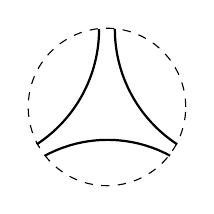
\begin{tikzpicture}[baseline=0]
        \draw[dashed] (0,0) circle (1);
        \draw[thick] (-0.1,0.99) arc (0:-56.8:1.75);
        \draw[thick] (0.1,0.99) arc (180:236.8:1.75);
        \draw[thick] (-0.79,-0.62) arc (118.5:61.6:1.67);
    \end{tikzpicture}
    }
\end{align*}
where
$$\scalebox{0.75}{
    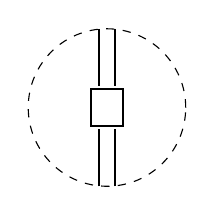
\begin{tikzpicture}[baseline=0]
        \draw[dashed] (0,0) circle (1);
        \node at (0,0) [thick,rectangle,draw] {$\phantom{2}$};
        \draw[thick] (-0.1, 1) -- (-0.1,0.27);
        \draw[thick] (0.1, 1) -- (0.1,0.27);
        \draw[thick] (-0.1, -1) -- (-0.1,-0.27);
        \draw[thick] (0.1, -1) -- (0.1,-0.27);
    \end{tikzpicture}} = 
    \scalebox{0.75}{
    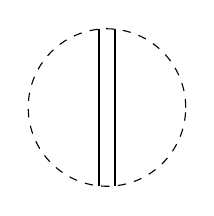
\begin{tikzpicture}[baseline=0]
        \draw[dashed] (0,0) circle (1);
        \draw[thick] (-0.1,1) -- (-0.1,-1);
        \draw[thick] (0.1,1) --(0.1,-1);
    \end{tikzpicture}} + \frac{1}{[2]} 
    \scalebox{0.75}{
    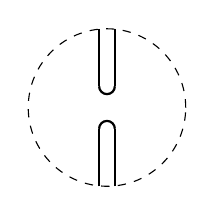
\begin{tikzpicture}[baseline=0]
        \draw[dashed] (0,0) circle (1);
        \draw[thick] (-0.1, 1) -- (-0.1,0.27);
        \draw[thick] (0.1, 1) -- (0.1,0.27);
        \draw[thick] (-0.1,0.27) arc (-180:0:0.1);
        \draw[thick] (-0.1, -1) -- (-0.1,-0.27);
        \draw[thick] (0.1, -1) -- (0.1,-0.27);
        \draw[thick] (-0.1,-0.27) arc (180:0:0.1);
    \end{tikzpicture}}
$$
is the Jones-Wenzl indempotent of the Temperley-Leib algebra
on two strands. In particular, this map is injective.
A reasonable question to ask then, is ``For what surfaces $\Sigma$ 
is the map $JW: S_q^Y(\Sigma) \to S_q(\Sigma)$ (defined in the same fashion)
injective?'' The following is a conjecture from the folklore:

\begin{conjecture*}[Folklore]
    For all $q \in \C^\times$ and oriented $\Sigma$, the map
    $JW: S_q^Y(\Sigma) \to S_q(\Sigma)$ is injective.
\end{conjecture*}

In this paper, we prove that this is true for all surfaces with
boundary. In so doing, we construct a finite presentations for
for the $\PGL_2$ skein algebra of the punctured torus and the
T-shirt. We also show that this conjecture is \emph{not} true 
in general by showing that the kernel of the $JW$ map for the
torus is one-dimensional. Moreover, we show that the $\PGL_2$
skein algebra of the torus is finitely generated and compute its
multiplication table. 